% Acceleration
\section{Acceleration}
	
% Acceleration -  Acceleration (a)
\subsection{Acceleration (a)}
Any change in velocity over a period of time is called acceleration. The sign (+ or -) of acceleration indicates it's direction. Acceleration can be…
\begin{itemize}
	\item speeding up
	\item speeding down
	\item turning
\end{itemize}

% Acceleration Graphs
\subsection{Acceleration Graphs}

% Graphs
\begin{figure}[H]%
	\hfill
	\subfigure[Zero Acceleration]{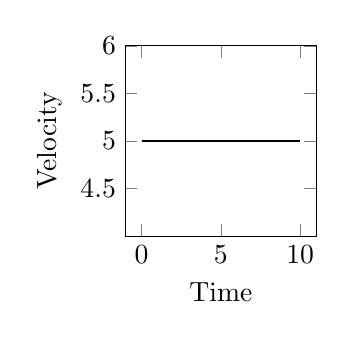
\begin{tikzpicture} \begin{axis}[xlabel = Time, ylabel = Velocity, width=4cm, height = 4cm] xmin = 0, xmax = 10, ymin = 0, ymax = 10, \addplot[domain = 0:10, smooth, thick] {5}; \end{axis} \end{tikzpicture}\label{fig:ZeroAcceleration}}
	\hfill
	\subfigure[Positive Acceleration]{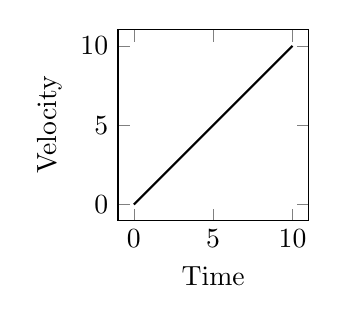
\begin{tikzpicture} \begin{axis}[xlabel = Time, ylabel = Velocity, width=4cm, height = 4cm] xmin = 0, xmax = 10, ymin = 0, ymax = 10, \addplot[domain = 0:10, smooth, thick] {x}; \end{axis} \end{tikzpicture}\label{fig:PositiveAcceleration}}
	\hfill
	\subfigure[Negative]{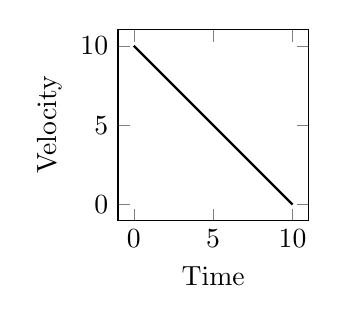
\begin{tikzpicture} \begin{axis}[xlabel = Time, ylabel = Velocity, width = 4cm, height = 4cm] xmin = 0, xmax = 10, ymin = 0, ymax = 10, \addplot[domain = 0:10, smooth, thick] {-x+10}; \end{axis} \end{tikzpicture}\label{fig:NegativeAcceleration}}
	\hfill
	\caption{Graphs of Acceleration}
	\label{fig:TypesofAccleration}
\end{figure}

As seen above in Figure \ref{fig:TypesofAccleration}, acceleration can be zero as seen in \ref{fig:ZeroAcceleration}, positive as seen in \ref{fig:PositiveAcceleration}, or negative as seen in \ref{fig:NegativeAcceleration}.
	
% Acceleration -  Uniform (Constant) Acceleration
\subsection{Uniform (Constant) Acceleration}
In Physics 1, we will generally assume that acceleration is \textit{constant}. With this assumption we are free to use this equation: \[a=\frac{\Delta v}{\Delta t}\] 
The SI unit of acceleration is the $m/s^2$.
	
% Acceleration -  Acceleration has a sign!
\subsection{Acceleration has a sign!}
If the sign of the velocity and the sign of the acceleration is the same, the object speeds up. If the sign of the velocity and the sign of the acceleration are different, the object slows down.